\section{Zhu's test function through a truncated reciprocal Xi transform}\label{zh:sec:extremal}

Zhu's proof of (Z3) takes $\widehat{f_0}(r)=B(r)h(r)$, with $B(r)=\prod_{0<\gamma_j\le T}(1-r^2/\gamma_j^2)$ a finite product over the ordinates up to a truncation height $T$, and a window kernel $h$ of type $a$. In the notation of Section~\ref{ch:clock}, $G(u)=\prod_{\gamma>0}(1+u/\gamma^2)$ is the reciprocal of the Laplace transform of the clock, which under RH is $\sum_{\gamma>0}e_\gamma/\gamma^2$. Truncate the product, $G_T(u)=\prod_{0<\gamma_j\le T}(1+u/\gamma_j^2)$. Then $1/G_T$ is the Laplace transform of the finite gamma convolution $\sum_{\gamma_j\le T}e_{\gamma_j}/\gamma_j^2$ and
\[
B(r)=G_T(-r^2),
\]
the reciprocal of that Laplace transform continued to the cut $s=-r^2$. Zhu's test function is the window kernel divided by the truncated reciprocal Xi transform on the cut. In the variable $t=r^2$ it vanishes at the Thorin atoms $\gamma_j^2\le T^2$ (and at the zeros of $h$), and under RH
\[
Q(f_0)=2\int_{t>T^2}h(\sqrt t)^2\,G_T(-t)^2\,U(dt).
\]
The optimisation is a trade: each atom killed costs a factor $r^2/\gamma_j^2$ of growth, which $h$ must absorb with its limited type.

We evaluated this family numerically (script \texttt{zh\_product\_bound.py}), with $h(r)=\bigl(\sin(ar/m)/(ar/m)\bigr)^m$, which has type $a$, optimising over the number $K$ of atoms killed and over the even exponent $m\ge2K+2$. Table~\ref{zh:tab:prod} is a computation of this chapter and not of Zhu. The quotient $Q(f_0)/\|f_0\|^2$ is evaluated on the zero side under RH, with the $1700$ ordinates of \texttt{data/zeros\_1700.txt} and an explicit Riemann von Mangoldt tail \cite{HSW22}, and on the geometric side by Zhu's formula \eqref{zh:Q}, which needs no hypothesis. The two agree to $13$ digits or more at $a=0.8$ and $1.0$ and to $3.5\times10^{-7}$ relative at $a=0.5$, where the tail beyond $1700$ ordinates limits the comparison, so every entry is an unconditional upper bound for $\lambda^{\rm even}_{\min}(\frac12,a)$.

\begin{table}[t]
\centering
\fitwidth{\begin{tabular}{rrrrrrr}
\toprule
$a$ & best bound & $K$ & $m$ & $\gamma_K$ & $N(T_*)$ & $T_*=2\pi e^{2a}$\\
\midrule
0.5 & $3.88\times10^{-4}$ & 2 & 6 & 21.0 & 1 & 17.1\\
0.8 & $4.03\times10^{-9}$ & 6 & 18 & 37.6 & 4 & 31.1\\
1.0 & $7.04\times10^{-14}$ & 9 & 26 & 48.0 & 8 & 46.4\\
\bottomrule
\end{tabular}}
\caption{The best Rayleigh quotient $Q(f_0)/\|f_0\|^2$ of Zhu's product family over the number $K$ of atoms killed and the even exponent $m$, with the optimal $K$ and $m$, the last ordinate $\gamma_K$ killed, the number $N(T_*)$ of ordinates below the resolution height $T_*=2\pi e^{2a}$ of Section~\ref{zh:sec:horizon}, and $T_*$ itself.}
\label{zh:tab:prod}
\end{table}

The product construction is crude. At $a=0.8$ it gives $4.03\times10^{-9}$ against about $1.7\times10^{-17}$ for the window infimum (the entry at $160$ modes of Table~\ref{zh:tab:hp}, an upper bound), and a general element of $PW_a$ does much better. The number of atoms worth killing grows with $a$ and exceeds the number $N(T_*)$ of ordinates below the horizon $T_*$ of the next section: in each row the last atom killed lies above $T_*$ and below $eT_*$. When $K$ is restricted to $N(T_*)$ the bound is worse by the factors $1.27$, $1.40$ and $1.05$. At $a=0.35$ and $a=1.2$ (not tabulated) the optimum is $K=0$ and $K=16$, equal to $N(T_*)$ in both cases. So atoms above the horizon are worth killing at the three tabulated half lengths, and three rows with $a\le1$ cannot settle the asymptotics (Zhu's Remark 13.6 in (Z3)).

\section{The Landau Widom horizon}\label{zh:sec:horizon}

Zhu's resolution height comes from a comparison of densities (his Section 9). By Jensen's formula a real entire function of exponential type $a$ has real zeros of average density at most $a/\pi$ on long intervals $[-R,R]$ about the origin, which Zhu takes as a bound for the local density, while the ordinates have density $\nu(t)=\frac1{2\pi}\log\frac t{2\pi}$ at height $t$. The two meet at
\begin{equation}\label{zh:horizon}
\frac a\pi=\frac1{2\pi}\log\frac T{2\pi}\iff T=T_*(a):=2\pi e^{2a},
\end{equation}
which we call the Landau Widom horizon, or the horizon. Zhu's argument is that below $T_*$ a test function of type $a$ can in principle interpolate the ordinates, placing a zero of $F$ on each of them, and that above $T_*$ the ordinates outnumber the available oscillations, so that $|F|^2$ must leak onto them. A count of degrees of freedom gives the same height up to a factor. An even function of $PW_a$ concentrated on the frequencies $[0,T]$ has about $aT/\pi$ degrees of freedom, since the time frequency rectangle $[-a,a]\times[-T,T]$ has about $2aT/\pi$ \cite{SlepianPollak61,LandauPollak62}, halved for evenness, while $N(T)\approx\frac T{2\pi}\log\frac T{2\pi e}$ ordinates lie below $T$. Equating the two counts gives $2\pi e^{2a+1}=eT_*$.

Zhu's decay law (Z4) uses $T_*$. He models the cost of killing $N(T_*)$ ordinates at saturated budget as an excursion of order $N(T_*)$ eigenvalues beyond the Shannon number of the window, at the plunge rate $\lambda_{K+j}\approx\exp(-\pi^2j/\log K)$ of the eigenvalues of the concentration operator of time and band limiting \cite{LandauWidom80}. This gives $-\log\lambda^{\rm even}_{\min}(\frac12,a)\asymp\pi^2N(T_*)/\log N(T_*)$ up to a constant, and the fit supplies the constant (his Section 9 and Conjecture 12.1). It is his model, fitted and not derived.

The passage from a window statement to a statement about the height of the zeros is a heuristic and not a theorem. Nothing in this book proves that positivity of Weil's form on every window of half length $a$ is implied by, or implies, the verification of the zeros up to a height of order $T_*(a)$, and Problem~\ref{zh:op:horizon} asks for the theorem that the heuristic would need.

A quadruple of off line zeros $\frac12\pm\delta\pm i\gamma$ contributes $4\re F(\gamma-i\delta)^2$ to $Q(f)$ for real even $f$, and a negative value of $Q$ needs a test function that nearly vanishes at the on line ordinates near $\gamma$ while keeping its energy near $\gamma\pm i\delta$. Heuristically this is possible only when the window has more degrees of freedom near $\gamma$ than the ordinates have, $a/\pi>\frac1{2\pi}\log\frac\gamma{2\pi}$, which predicts a detection threshold
\[
a_{\rm det}(\gamma,\delta)\approx\tfrac12\log\frac\gamma{2\pi}+O(1),
\]
with a weak dependence on $\delta$ for small $\delta$. Once the test function vanishes at the neighbours and at $\gamma$ itself, the contribution of the quadruple is $4\re F(\gamma-i\delta)^2=-4\delta^2F'(\gamma)^2+O(\delta^4)$, which is negative for small $\delta>0$, and it must exceed the residual of the on line zeros.

We tested this on a hypothetical configuration (scripts \texttt{zh\_detect.py} and \texttt{zh\_zeros.py}). Add to the on line zeros one quadruple $\frac12\pm\delta\pm i\gamma$, where $\gamma$ is the midpoint of the gap between two consecutive ordinates (numbers $10$ and $11$, $79$ and $80$, $649$ and $650$, $1517$ and $1518$). The matrix is the zero side formula of Theorem~\ref{yo:thm:lowner} for Yoshida's form on $C(a)$, with the first $2100$ ordinates (the last at $2620.28$) and the modes $|n|\le\lceil a(\gamma+45)/\pi\rceil+2$, whose frequencies $\pi n/a$ reach $45$ beyond the height of the quadruple. The on line zeros contribute a positive semidefinite Gram matrix and the quadruple a real symmetric matrix of rank at most four, so any negativity comes from the quadruple. Two criteria are used. In criterion (i) the entry is the smallest $a$ on a grid of step $0.05$ at which the least eigenvalue of the float64 matrix is below $-10^{-11}$. In criterion (ii) it is the smallest $a$ at which the exact least eigenvalue is negative, which is decided in ball arithmetic: in each parity sector the quadruple is a perturbation of rank two of a positive definite matrix, so the sign is decided by a two by two determinant. At the heights $1000.57$ and $1999.99$ criterion (ii) is only an upper bound, from the principal submatrix on the modes with $|\pi n/a-\gamma|\le150$: by interlacing a detection there is a detection for the full matrix, and a failure to detect proves nothing. The entry of the table is the smaller of this band value and the entry of criterion (i).

The rounding error of the float64 eigenvalue is bounded a priori, from the rounding of the Gram matrix and a textbook bound for the eigensolver, by $4\times10^{-12}$ to $5\times10^{-12}$ at height $51$, $9\times10^{-12}$ at $200$, about $2.6\times10^{-11}$ at $1000$ and $4\times10^{-11}$ at $2000$. The cut $-10^{-11}$ of criterion (i) is therefore safe in double precision at the heights $51$ and $200$, whereas at $1000$ and $2000$ the bound exceeds the cut, so that there a detection is certified only when the float64 eigenvalue lies below minus the bound. At the printed value of $a$ every one of the sixteen events is certified: in fourteen cells by the float64 eigenvalue and this bound, in the other two (at $(51.37,0.01)$ and $(199.64,0.2)$) by the exact test of the cut. The grid point below the printed value is certified as a non detection at the heights $51$ and $200$ only. Each entry of criterion (i) is an upper bound, for the model of the table, for the sign change in exact arithmetic.

\begin{table}[t]
\centering
\fitwidth{\begin{tabular}{rrrrrr}
\toprule
$\gamma$ & $\frac12\log\frac\gamma{2\pi}$ & $\delta=0.01$ & $\delta=0.05$ & $\delta=0.2$ & $\delta=0.45$\\
\midrule
\multicolumn{6}{l}{Criterion (i): the float64 least eigenvalue falls below $-10^{-11}$}\\
51.37 & 1.051 & 1.20 & 1.15 & 1.15 & 1.10\\
199.64 & 1.729 & 1.85 & 1.80 & 1.75 & 1.75\\
1000.57 & 2.535 & 2.65 & 2.65 & 2.60 & 2.50\\
1999.99 & 2.882 & 3.05 & 3.00 & 2.95 & 2.45\\
\midrule
\multicolumn{6}{l}{Criterion (ii): the exact least eigenvalue is negative}\\
51.37 & 1.051 & 1.05 & 1.00 & 0.95 & 0.95\\
199.64 & 1.729 & 1.55 & 1.50 & 1.50 & 1.50\\
1000.57 & 2.535 & $\le2.65$ & $\le2.65$ & $\le2.60$ & $\le2.50$\\
1999.99 & 2.882 & $\le3.05$ & $\le3.00$ & $\le2.95$ & $\le2.45$\\
\bottomrule
\end{tabular}}
\caption{Smallest window half length $a$ at which Yoshida's form on $[-a,a]$ detects a hypothetical off line quadruple $\frac12\pm\delta\pm i\gamma$ added to the first $2100$ zeros, on a grid of step $0.05$ (script \texttt{code/zh\_detect.py}, record \texttt{data/zh\_detect.json}). The entries of the lower block are exact on the full matrix at the heights $51.37$ and $199.64$; at $1000.57$ and $1999.99$ the entries marked $\le$ are upper bounds, the smaller of the value from a band of modes and the entry of criterion (i) above. At the cell $(1999.99,0.2)$ the band computation of $150$ modes does not detect the quadruple at $2.90$ and $2.95$ (it does at $3.00$, with $2100$, $4000$ and $8000$ zeros and with the margin $90$ in place of $45$ in the number of modes), so that the entry $2.95$ there is the entry of criterion (i); the exact test detects the quadruple in a band of $300$ modes at $2.95$ and in a band of $600$ modes at $2.90$.}
\label{zh:tab:det}
\end{table}
% CHECK: Table zh:tab:det, criterion (ii) at 1000.57 and 1999.99 is an upper bound (the smaller of the band 150 value and the certified entry of criterion (i), finding M8 of misc/reviews/nick-zhu/final-Z18.md): the full matrices there are PENDING, the cluster run of 17 October 2026 (data/zh_detect.json, misc/reviews/nick-zhu/checks-Z2.md sections 5 and 7) having gone to bands of 600 modes at delta = 0.01 and 0.2 only. Everything else the table needs is settled by that run: its 32 entries agree.

\begin{figure}[t]
\centering
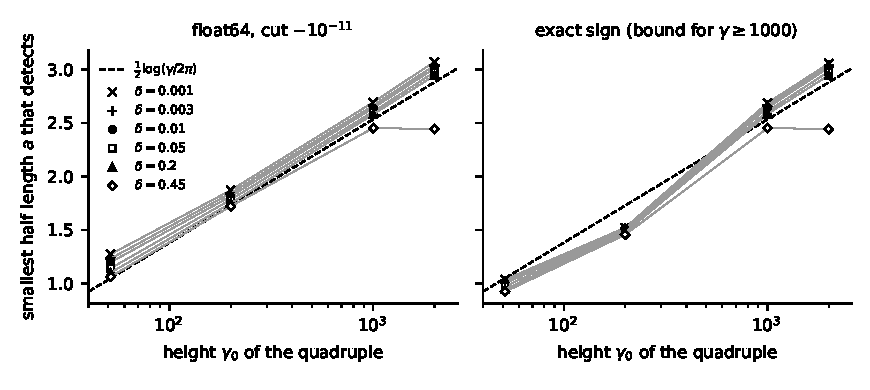
\includegraphics[width=0.92\textwidth]{fig/zh_horizon.pdf}
\caption{Detection thresholds of Table~\ref{zh:tab:det} and of the displacements $\delta=0.001$ and $0.003$ of the text against the height $\gamma$ of the hypothetical quadruple (logarithmic axis), for $\delta=0.001$, $0.003$, $0.01$, $0.05$, $0.2$, $0.45$ (points of equal $\delta$ joined), with the horizon $\frac12\log(\gamma/2\pi)$ dashed; the vertical axis is the half length $a$ of the window. Left: criterion (i). Right: criterion (ii), with upper bounds at the heights $1000$ and $2000$. The points are the thresholds refined by bisection to $0.005$, so that they lie up to $0.05$ below the entries of the table. Drawn by \texttt{code/zh\_detect.py} (option \texttt{--figure}) from \texttt{data/zh\_detect.json}.}
\label{zh:fig:horizon}
\end{figure}

For $\delta\le0.2$ every threshold of criterion (i) lies $0.02$ to $0.17$ above $\frac12\log(\gamma/2\pi)$. For $\delta=0.45$ it lies above it by $0.05$ and $0.02$ at the heights $51$ and $200$ and below it by $0.04$ and $0.43$ at the heights $1000$ and $2000$ (Figure~\ref{zh:fig:horizon}). Refined by bisection to $0.005$ the thresholds of criterion (ii) are $1.003$, $0.975$, $0.947$, $0.925$ at $\gamma=51.37$ and $1.506$, $1.491$, $1.478$, $1.456$ at $\gamma=199.64$, for $\delta=0.01$, $0.05$, $0.2$, $0.45$, which lie below the horizon by $0.05$ to $0.13$ and by $0.22$ to $0.27$. So the horizon is neither an upper bound nor a lower bound for the detection threshold in these data. The table is set by the cut and by the model as much as by the horizon: near the cut the negative eigenvalue grows by a factor $2\times10^2$ to $2\times10^4$ per step $0.05$ in $a$, so that any cut between $10^{-16}$ and $10^{-9}$ moves the thresholds by less than $0.15$, but double precision cannot see the sign change itself, because between the exact sign change and the cut the float64 eigenvalue is rounding noise (between $-2\times10^{-15}$ and $-5\times10^{-15}$ for every $a$ from $1.3$ to $1.7$ at height $200$).

The dependence on $\delta$ is weak for small $\delta$. At $\delta=0.001$ the thresholds of criterion (i) are $1.30$, $1.90$, $2.70$, $3.10$ at the four heights, and at $\delta=0.003$ they are $1.25$, $1.85$, $2.70$, $3.05$. From $\delta=0.001$ to $0.2$ they fall by $0.10$ to $0.15$, and they are nonincreasing in $\delta$ in every row. So a displacement of $0.01$ is detected almost as early as one of $0.2$, but a displacement of $0.45$ is detected at height $2000$ much earlier than the horizon suggests. The weak dependence is a property of these computations and not a consequence of the expansion above. What lets a large displacement be seen early is the growth of a test function off the real axis: for $F\in PW_a$ bounded on $\R$, the Phragm\'en Lindel\"of bound gives $|F(\gamma-i\delta)|^2\le e^{2a\delta}\sup_\R|F|^2$, which is $9.1$ at $a=2.45$, $\delta=0.45$. It is an upper bound and not a measured gain, and the data are consistent with the reading that at height $2000$ the term of the quadruple, amplified by up to that factor, can beat on line neighbours spaced about $0.9$ apart (the gap that contains the quadruple is $0.889$, the mean spacing $1.09$) before the window resolves them individually. The experiment does not test this reading.

Three features of the model limit what the table says. First, the configuration is not count preserving. The variant that removes the two on line zeros flanking the gap is detected earlier, by $0.15$ to $0.30$ in each of the eight cells computed ($\delta=0.01$ and $0.2$ at the four heights), and every one of its thresholds lies at or below the horizon, by $0.03$ to $0.24$. The thresholds of the table are therefore those of a configuration with two extra zeros and not a statement about a configuration with the true zero count. Second, the truncation to $2100$ ordinates can only advance detection, because the omitted zeros add positive semidefinite terms. In the eight cells that were also run with $4000$ and with $8000$ ordinates the float64 thresholds are unchanged, but the rounding bound grows with the number of zeros, and the entry $(1999.99,0.2)$ is no longer certified at either size (the certified value is $3.00$), nor is $(1000.57,0.01)$ at $8000$. Third, with the margin $90$ in place of $45$ in the number of modes the entry $(1999.99,0.01)$ is $3.00$ and not $3.05$.

Compare the tent coefficient $D(x)=x\langle\chi_0,\chi_0\rangle$ of Chapter~\ref{chap:yoshida} at the level $x=2a$. By Remark~\ref{yo:rem:scale} it turns negative near $x_*\approx(2\log\gamma+\log p_1)/\delta$, with $p_1=\sum_{\gamma>0}\gamma^{-2}=0.0231049931$. The tent is one vector of the window $C(a)$, so $x_*/2$ is only an upper bound for the half length at which the window detects the quadruple. For $\delta=0.2$ the level at which the quadruple can first push $D$ negative for some phase, computed from the first $8000$ ordinates, gives $x_*/2=8.68$, $16.2$, $24.2$, $27.8$ at the four heights, against the thresholds $1.15$, $1.75$, $2.60$, $2.95$ of Table~\ref{zh:tab:det}. Over the $16$ cells of the table the window thresholds are $4.0$ to $177$ times smaller than $x_*/2$, the ratio being roughly $2/\delta$ ($144$ to $177$ at $\delta=0.01$, $29$ to $37$ at $0.05$, $7.5$ to $9.4$ at $0.2$ and $4.0$ to $5.1$ at $0.45$). The formula for $x_*$ overestimates the computed level by $2$ to $22$ percent. The window data do not support an order $\delta^{-1}\log\gamma$ for the window threshold itself. For the height $3\times10^{12}$ the formula gives $x_*/2=26.85/\delta$, that is $59.7$ at $\delta=0.45$ and $134$ at $\delta=0.2$, against the half length $13.45$ of the horizon, with the same ratio $2/\delta$. Proposition~\ref{yo:prop:barrier} (level $47$) is proved for $D$ only, and Table~\ref{zh:tab:det} shows that the window is far more sensitive than the coefficient. The level $47$ is therefore not the level at which windows begin to see beyond the verification of the zeros, and the conversion from half lengths to levels, here and in Chapter~\ref{chap:yoshida}, is a heuristic.
% CHECK: the values 26.85/delta, 59.7 and 134 for the height 3e12 come from the formula of Remark yo:rem:scale and are not a computation.

The horizon turns a window statement into a height statement only heuristically, and only for small displacements. Large displacements are seen below the horizon at the heights $1000$ and $2000$ (Table~\ref{zh:tab:det}), and if the margin below the horizon keeps growing beyond the range tested, a window of half length near $13$ could see a large displacement far above $3\times10^{12}$. Table~\ref{zh:tab:heights} lists the heights $2\pi e^{2a}$ of some window statements.

\begin{table}[t]
\centering
\fitwidth{\begin{tabular}{lrr}
\toprule
window statement & half length $a$ & height $2\pi e^{2a}$\\
\midrule
Yoshida's Theorem 1, as Zhu reports it & $0.347$ & $12.6$\\
Zhu's certificate (Z2) & $0.8$ & $31.1$\\
practical limit of envelope certificates, Zhu's Remark 1.6 & $\approx1.6$ & $154$\\
verification of the zeros to $3\times10^{12}$ \cite{PT21} & $\approx13.4$ & $3\times10^{12}$\\
RH & $\infty$ & $\infty$\\
\bottomrule
\end{tabular}}
\caption{The horizon $2\pi e^{2a}$ at the half lengths of some window statements, and the half length $\frac12\log(H/2\pi)=13.45$ at which it equals the height $H=3\times10^{12}$ of the verification of the zeros. The conversion is a heuristic and not a theorem.}
\label{zh:tab:heights}
\end{table}

Yoshida's window lies below the first ordinate: its height $4\pi=12.57$ is less than $\gamma_1=14.13$. Zhu's certificate reaches about the fourth ordinate ($\gamma_4=30.42<31.12<\gamma_5=32.94$). Under the heuristic, a statement about these windows speaks about the zeros below the height shown, which the verification of the zeros covers far beyond.
